\documentclass[a4paper, 14pt]{extarticle}
\usepackage[a4paper, nohead, left=30mm, right=20mm, top=20mm, bottom=20mm]{geometry}
\usepackage[english, russian]{babel}
\usepackage[T1, T2A]{fontenc}
\usepackage[utf8x]{inputenc}
\usepackage{amsthm}
\usepackage{amssymb}
\usepackage{float}
\usepackage{graphicx}
\usepackage[ruled]{algorithm}
\usepackage{algorithmic}
\usepackage{array}
\usepackage{lscape}
\usepackage{ulem}

\graphicspath{{../figures/eps/bw/}}

%\linespread{1.3}
%\renewcommand{\rmdefault}{ftm}

\def\figureref#1{Рис.\,\protect\ref{#1}}
\def\eqref#1{(\protect\ref{#1}\protect)}

\floatname{algorithm}{Алгоритм}
\theoremstyle{plain}
\newtheorem{theorem}{Теорема}
\newtheorem{lemma}{Лемма}
\theoremstyle{definition}
\newtheorem{definition}{Определение}

\begin{document}
	\Russian

	\begin{titlepage}
{
	\newpage
	\fontsize{14pt}{22pt}

	\begin{center}
	{
		\fontsize{12pt}{20pt} \sf
		\mbox{ УЧРЕЖДЕНИЕ РОССИЙСКОЙ АКАДЕМИИ НАУК }\\[5pt]
		\mbox{ САНКТ-ПЕТЕРБУРГСКИЙ АКАДЕМИЧЕСКИЙ УНИВЕРСИТЕТ –- НАУЧНО- }\\
		\mbox{ ОБРАЗОВАТЕЛЬНЫЙ ЦЕНТР НАНОТЕХНОЛОГИЙ РАН }
	}
	\end{center}

	\vspace{20pt}
	\hfill
	\begin{minipage}{220pt}
		\begin{center}
		{
			\fontsize{12pt}{20pt}
			На правах рукописи\\[15pt]
			Диссертация допущена к защите\\
			Зав. кафедрой\\
			\vspace{10pt}
			\hspace{10pt}\hrulefill\hspace{10pt} \\
			\vspace{5pt}
			\hspace{25pt} ``\hspace{20pt}'' \hrulefill\hspace{5pt}2010 г. \hspace{25pt}
		}
		\end{center}
	\end{minipage}

	\vspace{30pt}
	\begin{center}
	{
		{ \bf ДИССЕРТАЦИЯ } \\
		{ НА СОИСКАНИЕ УЧЕНОЙ СТЕПЕНИ } \\[5pt]
		{ \bf МАГИСТРА } \\
	}
	\end{center}

	\vspace{10pt}
	\begin{flushleft}
	{
		Тема: Алгоритмическое перечисление альтернированных $k$-танглов \\
		\vspace{10pt}
		Направление: 010600.68 –- Прикладные математика и физика \\
		\vspace{10pt}
		Магистерская программа: ``Математические и информационные технологии'' \\
	}
	\end{flushleft}

	\vspace{20pt}
	\begin{flushleft}
		{ Выполнил студент \hfill А. С. Мишунин} \\
		\begin{center} { \fontsize{8pt}{0pt} (подпись) } \end{center}
		{ Руководитель:\\д. ф. - м. н., профессор \hfill А. В. Омельченко} \\
		\begin{center} { \fontsize{8pt}{0pt} (подпись) } \end{center}
		{ Рецензент:\\к. ф. - м. н., доцент \hfill В. Р. Мешков}
		\begin{center} { \fontsize{8pt}{0pt} (подпись) } \end{center}
	\end{flushleft}

	\vfill
	\begin{center}
	{
		Санкт-Петербург \\[5pt]
		2010 г.
	}
	\end{center}
}
\end{titlepage}

	\setcounter{page}{2}

	\newpage
\renewcommand{\abstractname}{Реферат}
\begin{abstract}
	Данная работа состоит из введения, трех глав основной части, заключения и списка литературы. Написана на 30 листах.
	Содержит 23 иллюстрации, 4 таблицы и 3 листинга алгоритма. Список литературы содержит 19 наименований.

	Результатом работы является описание алгоритма, который позволяет генерировать все возможные простые связные
	альтернированные $k$-танглы с количеством перекрестков, не превосходящим заданное число. Основными его достоинствами
	по сравнению с аналогичными для узлов и зацеплений являются отсутствие необходимости в больших хеш-таблицах, малый по
	сравнению с общим количеством генерируемых объектов объем необходимой памяти со случайным доступом и малый объем
	выполняемой заведомо бесполезной работы.
	
	Также в работе описан алгоритм рисования диаграмм $k$-танглов.

	%\listoffigures
	%\listoftables
	%\listofalgorithms
\end{abstract}


	\newpage
	\renewcommand{\contentsname}{Оглавление}
	\tableofcontents

	\newpage
\section{Введение}

	\subsection{Некоторые определения}

	\begin{figure}[ht]
		\centering
		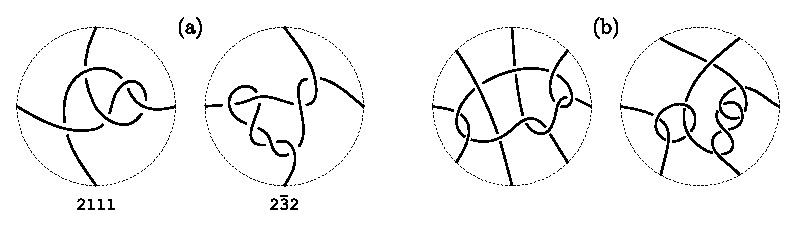
\includegraphics{c/tangles-example.eps}
		\caption{$2$-танглы (a), $k$-танглы в общем случае (b)\label{figure:tangles-example}}
	\end{figure}

	\begin{definition}
		\label{definition:tangle}
		$k$-танглом называется гладкое вложение $k$ отрезков и конечного числа окружностей в $B^3$
		(трехмерный замкнутый шар единичного радиуса), если $2k$ концов отрезков взаимно однозначно отображаются
		на точки с координатами $(\cos\pi i/k, \sin\pi i/k, 0)$, $i\in\{0, 1, \dots, 2k{-}1\}$, называемые
		концами $k$-тангла, и больше ни какие точки отрезков или окружностей на границу $B^3$ не отображаются.
	\end{definition}

	\begin{definition}
		\label{definition:tangle-equiv}
		$k$-танглы $T_1$ и $T_2$ называются эквивалентными, если существует изотопия $B^3$, сохраняющая границу
		неподвижной, которая переводит $T_1$ в $T_2$.
	\end{definition}

	\begin{definition}
		$k$-танглы $T_1$ и $T_2$ называются слабо эквивалентными, если существует изотопия $B^3$ (не обязательно
		сохраняющая границу неподвижной) которая переводит $T_1$ в $T_2$.
	\end{definition}

	\begin{figure}[ht]
		\centering
		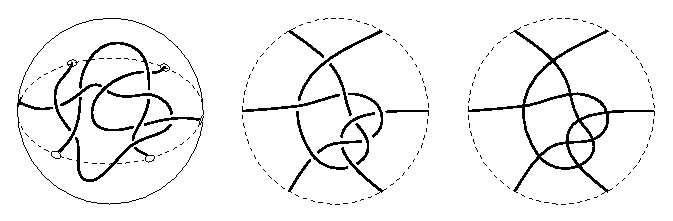
\includegraphics{c/tangle-diagram-projection.eps}
		\caption{$3$-тангл, его диаграмма и проекция\label{figure:3-tangle-and-proj}}
	\end{figure}

	Аналогично узлам и зацеплениям мы можем ввести понятие диаграммы и для $k$-танглов, строя невырожденные проекции
	$k$-тангла на плоскость, проходящую через его концы. Из \figureref{figure:tangles-example} \figureref{figure:3-tangle-and-proj}
	можно получить интуитивное представление о том, что такое диаграммы; строгое определение и подробное обсуждение
	``тонких мест'', напрямую не относящихся к нашей текущей теме, читатель может найти, например, в книге \cite{Cromwell2004}.
	Диаграммы, которые отличаются только плоской изотопией, сохраняющей граничную окружность, мы различать не будем.

	\begin{definition}
		Перекрестками диаграммы (проекции) называются точки, в которые проецируются две точки $k$-тангла. Ребрами
		диаграммы (проекции) называются максимальные множества точек, не лежащие на границе, в которые проецируется
		только по одной точке $k$-тангла.
	\end{definition}

	Ребра гомеоморфны открытым отрезкам и соединяют либо 2 перекрестка, либо 2 конца $k$-тангла либо конец с перекрестком.

	\begin{definition}
		Минимальной диаграммой $k$-тангла $T$ называют диаграмму $T$ с минимальным количеством перекрестков.
	\end{definition}

	\begin{figure}[ht]
		\centering
		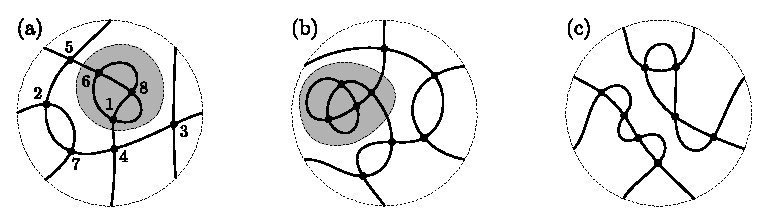
\includegraphics{c/composite-non-connected-projections.eps}
		\caption{Составные (a, b) и несвязные (c) проекции\label{figure:composite-proj}}
	\end{figure}

	\begin{definition}
		Диаграмма (проекция) $k$-тангла называется составной, если строго внутри граничной окружности существует замкнутая
		гладкая несамопересекающаяся кривая, которая трансверсально пересекает диаграмму ровно в двух точках и содержит
		внутри как минимум один перекресток. В противном случае диаграмма называется простой.
	\end{definition}

	\begin{definition}
		$k$-тангл называется простым, если просты все его минимальные диаграммы.
	\end{definition}

	\begin{definition}
		Диаграмма (проекция) называется связной, если граф, ребрами которого являются ребра диаграммы (проекции), а
		вершинами --- вершины и концы диаграммы (проекции), является связным.
	\end{definition}

	\begin{definition}
		$k$-тангл называется связным, если связна любая его диаграмма.
	\end{definition}

	\begin{definition}
		Диаграмма $k$-тангла называется альтернированной, если у каждого ребра, соединяющего два перекрестка, один из
		концов проходит над перекрестком, а другой --- под.
	\end{definition}

	\begin{definition}
		$k$-тангл называется альтернированным, если он имеет альтернированную диаграмму.
	\end{definition}


	\subsection{Постановка задачи}

	Как и в случае с узлами и зацеплениями, было бы логично поставить задачу классификации и для $k$-танглов. На настоящий
	момент результаты в этой области имеются в основном только для $2$-танглов. Общий случай уже интересен сам по себе,
	более того $k$-танглы могут оказаться полезными для исследованиях в других областях, например, для представления узлов
	и зацеплений в замкнутых ориентируемых поверхностях произвольного рода \cite{Kauffman1999, Kuperberg2003} --- так называемых
	виртуальных узлов и зацеплений.

	Так в работе \cite{Conway1970} J.~Conway ввел понятие танглов (которые в соответствии с Определением~\ref{definition:tangle}
	являются $2$-танглами) в качестве средства для описания и классификации узлов и зацеплений. Там же была предложено разделение
	танглов на классы рациональных, алгебраических и трансцендентных. Самым поддающимися исследованию оказались рациональные
	танглы --- для них проблема классификации была полностью решена \cite{KauffmanLambropoulou2004}.

	Для простых альтернированных $2$-танглов было получено полиномиальное уравнение на производящую функцию
	\cite{SundbergThistlethwaite1998}, которое затем было использовано там же для улучшения оценок на количество простых
	альтернированных зацеплений.

	Матричные интегралы рассматриваются как средство для перечисления альтернированных $k$-танглов в
	\cite{Justin1999_1, Justin1999_2, JustinZuber2000, Justin2001, JacobsenJustin2002, JustinZuber2003}.
	Там приведены теоретические результаты,	а также численно полученная таблица количеств простых альтернированных 
	$2$- и $3$-танглов. Однако сложность предложенного метода быстро растет с увеличением $k$.

	Наконец в \cite{KanenobuSaitoSatoh2003} с точностью до слабой эквивалентности были классифицированы простые $2$-танглы
	не более, чем с семью перекрестками.

	Целью данной работы является алгоритм, позволяющий получить все альтернированные $k$-танглы (а точнее их минимальные диаграммы)
	с количеством перекрестков, не превосходящим заданное число. Иными словами проделать то же самое для альтернированных танглов,
	что было сделано в \cite{Rankin2002_1, Rankin2002_2, Rankin2002_3} для альтернированных зацеплений. Однако, класс рассматриваемых
	$k$-танглов стоит ограничить уже по той причине, что всего их, даже с конечным числом перекрестков, бесконечное число. Поэтому
	мы будем рассматривать только связные альтернированные танглы. Также из рассмотрения традиционно исключаются составные
	диаграммы --- так мы и будем поступать.

	Выбор класса альтернированных $k$-танглов обусловлен рядом их известных свойств, сильно облегчающих задачу. В частности,
	любая минимальная диаграмма простого альтернированного тангла является альтернированной и, кроме того, все его минимальные диаграммы
	могут быть получены друг из друга применением (возможно, многократным) преобразования, называемого ``flype''
	(см. \figureref{figure:flype}). Также любая нередуцируемая (т. е. такая, в которой нельзя сразу же ``распутать'' петлю
	первым движением Редемейстера, тем самым уменьшив число перекрестков), в частности --- простая, альтернированная диаграмма
	является минимальной диаграммой.

	\begin{figure}[ht]
		\centering
		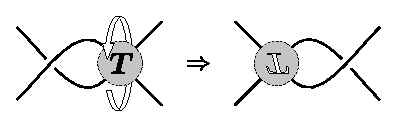
\includegraphics{c/flype.eps}
		\caption{Flype\label{figure:flype}}
	\end{figure}

	P.~G.~Tait более 100 лет назад \cite{Tait1900} выдвинул предположение о возможности получения минимальных альтернированных диаграмм
	узлов и зацеплений друг из друга с помошью преобразования \figureref{figure:flype}, получившее название ``Tait flyping conjecture''.
	Доказано оно было относительно недавно W.~Menasco и M.~Thistlethwaite в \cite{MenascoThistlethwaite1991, MenascoThistlethwaite1993},
	а утверждения выдвинутые выше являются являются его простыми обобщениями и следствиями.

	Как правило в литературе (в нашем случае это во всех ссылках, кроме \cite{KanenobuSaitoSatoh2003}) для перечисления танглов
	используются аналитические методы, поэтому там используется Определение~\ref{definition:tangle-equiv} для определения эквивалентности
	двух $k$-танглов, так как оно дает наиболее простые соотношения. Мы, однако, собираемся явно получать проекции всех простых связных
	альтернированных $k$-танглов с количеством перекрестков не превосходящим заданное число, значит заинтерисованы в максимальном сокращении
	количества ненужной работы. Поэтому имеет смысл отождествлять две диаграммы $k$-танглов, отличающиеся действием элемента
	группы $D_{2k}$ в дополнение к разрешенным Определением~\ref{definition:tangle-equiv} преобразованием. Очевидно, что большая часть
	танглов несимметрична, поэтому уже для $2$-танглов мы получаем выигрыш почти в 8 раз, а с ростом $k$ он становится все более
	значительным.

	Схема дальнейшей части работы выглядит следующим образом: в Главе~\ref{section:projections} мы рассмотрим алгоритм генерации
	всех возможных неэквивалентных (с точностью до плоской изотопии и $D_{2k}$) простых связных проекций $k$-танглов, затем мы
	покажем как модифицировать его для генерации простых альтернированных танглов в Главе~\ref{section:alternating}. Наконец,
	в Главе~\ref{section:drawing} приводится алгоритм создания ``красивых'' изображений $k$-танглов, который, конечно,
	непосредственного отношения к рассматриваемым вопросам не имеет, но является настолько полезным в процессе исследования, что
	фактически без него невозможно обойтись.

	\newpage
\section{Перечисление проекций $k$-танглов}
	\label{section:projections}

		Как и было сказано выше, в данной главе будет дано описание алгоритма, перечисляющего простые связные проекции
		$k$-танглов с количеством перекрестков, не превосходящим заданное число. Проекции считаются одинаковыми, если
		одну можно перевести в другую композицией плоской изотопии и элемента группы $D_{2k}$, то есть если они гомеоморфны.

	\subsection{Элементарные операции с проекциями}
		\label{subsection:cutting}

		\begin{definition}
			Перекресток проекции называется пограничным, если он соединен одним из ребер проекции с одним из ее концов.
		\end{definition}

		\begin{definition}
			Удалением пограничного перекрестка проекции называется операция, при которой выбранный перекресток
			удаляется из проекции вместе с ребрами, соединяющими его с концами проекции, а ребра, которые раньше
			соединяли удаленный перекресток с остальной частью проекции, теперь соединяют остальную часть с новыми
			концами проекции. При этом требуется, чтобы удаляемый перекресток был соединен с каким-либо другим
			перекрестком проекции. Число концов проекции может при этом меняться на $0$, $2$, или $-2$. Обратная
			операция называется приклеиванием пограничного перекрестка. 
		\end{definition}

		\begin{figure}[ht]
			\centering
			\includegraphics{c/geneology.eps}
			\caption{Последовательные удаления перекрестков\label{figure:geneology}}
		\end{figure}

		К любой проекции, удовлетворяющей нашим условиям и содержащей перекрестки, мы можем последовательно применять операцию
		удаления пограничного перекрестка как на \figureref{figure:geneology}, вопрос лишь в том, можно ли это делать так,
		чтобы в конце всегда получалась проекция из одного перекрестка, а все промежуточные проекции были просты и связны.
		Или, иными словами, любую ли простую связную простую проекцию с перекрестками можно получить из проекции, состоящей
		из одного перекрестка, последовательными приклеиваниями пограничного перекрестка так, чтобы все промежуточные проекции
		были простые и связные. Ответ здесь положительный, благодаря Теореме~\ref{theorem:good-cutting}.

		\begin{theorem}
			\label{theorem:good-cutting}
			В любой связной простой проекции $k$-тангла, содержащей более одного перекрестка, можно удалить пограничный
			перекресток так, чтобы получившаяся в результате проекция была простой и связной.
		\end{theorem}
		\begin{proof}
			Простота любой получающейся проекции очевидна. Осталось доказать возможность получения связной проекции, показав,
			что среди пограничных перекрестков найдется не являющийся точкой сочленения проекции. Точка сочленения --- перекресток,
			через которую можно провести хорду (гладкую несамопересекающуюся кривую, только начало и конец которой лежат на граничной
			окружности), которая больше нигде с проекцией не пересекается, и с обеих сторон от которой есть перекрестки.
			\begin{figure}[H]
				\centering
				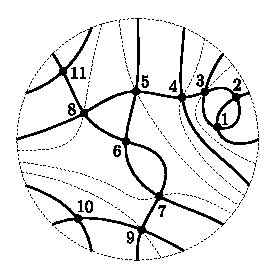
\includegraphics{c/cutpoints-proof.eps}
				\caption{К доказательству Теоремы~\ref{theorem:good-cutting}\label{figure:cutpoints-proof}}
			\end{figure}
			Проведем через все точки сочленения проекции соответствующие хорды таким образом, чтобы они все не пересекались
			(легко доказать, что так всегда можно сделать) как на \figureref{figure:cutpoints-proof}. Каждая из хорд
			делит круг на две части, и всегда за конечное число шагов найдется ``крайняя'' хорда, у которой точки сочленения
			есть только по одну сторону. Но перекрестки там есть по определению точки сочленения, значит есть и пограничные
			перекрестки, так как диаграмма простая.
		\end{proof}

		Исходя из вышеприведенных утверждений, уже можно предложить следующий алгоритм: обозначим за $P_n$ множество всех
		связных простых проекций с $n$ перекрестками, за $P_1$ возьмем множество из единственной проекции с одним перекрестком.
		Имея $P_n$, вычислим $P_{n+1}$ следующим образом: возьмем мультимножество результатов всех возможных приклеиваний
		пограничного перекрестка ко всем проекциям из $P_n$ и удалим из него дубликаты и составные проекции.

		Однако, этот алгоритм не очень хорош, так как содержит трудоемкую стадию удаления дубликатов. Ниже будет показано, как
		от нее избавится.

	\subsection{Инвариант помеченных проекций}
		\label{subsection:root-code}

		\begin{definition}
			Помеченной проекцией называется связная проекция $k$-тангла, снабженная тройкой $r = (v, e, f)$, где $v$ ---
			перекресток проекции, $e$ --- ребро проекции, инцидентное $v$ и $f$ --- грань проекции, инцидентная $v$ и $e$.
			$v$ назовем помеченным перекрестком, $e$ --- помеченным ребром и $f$ --- помеченной гранью.
		\end{definition}

		Положение грани $f$ относительно перекрестка $v$ и ребра $e$ задает направление обхода, которое может быть по часовой
		стрелки и против часовой стрелки.

		Построим теперь инвариант помеченной $(v, e, f)$ проекции $P$ (который мы назовем ``root-code'') следующим образом
		(см. Алгоритм~\ref{algorithm:root-code} и \figureref{figure:rcode-example}):

		\begin{algorithm}[H]
			\caption{root-code$(P, (v, e, f))$\label{algorithm:root-code}}
			\algsetup{linenosize=\small, linenodelimiter=.}
			\begin{algorithmic}[1]
				\STATE $A \leftarrow \{\}$
				\STATE $free \leftarrow 2$

				\STATE $Q \leftarrow \{v\}$
				\STATE $number[v] \leftarrow 1$
				\STATE $incoming[v] \leftarrow e$

				\WHILE{$Q \neq \varnothing$}
					\STATE $u \leftarrow head[Q]$
					\STATE $dequeue(Q)$

					\FOR{(для) всех ребер $(u, w) \in P$ в порядке, заданном $f$, начиная с $incoming[u]$}
						\IF{$w$ --- конец диаграммы}
							\STATE $code \leftarrow 0$
						\ELSE
							\IF{$number[w]$ не определен}
								\STATE $number[w] \leftarrow free$
								\STATE $free \leftarrow free + 1$
								\STATE $enqueue(Q, w)$
							\ENDIF
							\STATE $code \leftarrow number[w]$
						\ENDIF

						\STATE $push(A, code)$
					\ENDFOR
				\ENDWHILE

				\RETURN $A$
			\end{algorithmic}
		\end{algorithm}

		\begin{figure}[ht]
			\centering
			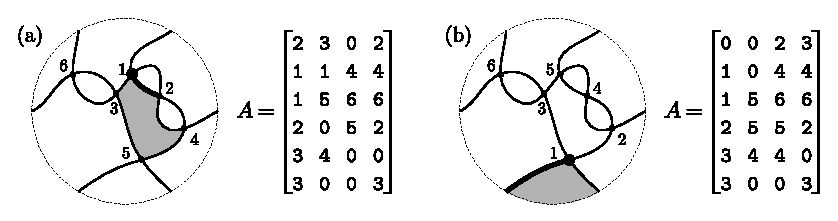
\includegraphics{c/rcode-example.eps}
			\caption{Примеры вычисления root-code\label{figure:rcode-example}}
		\end{figure}

		Результатом работы алгоритма будет последовательность, в которой на каждый перекресток проекции $P$ приходится по 4 числа ---
		номера соседних перекрестков в порядке обхода, заданном гранью $f$, или $0$, если данный сосед является концом диаграммы.
		Номера присваиваются перекресткам начиная с единицы в порядке обхода в ширину. В инварианте вершины описаны также в порядке
		возрастания номера.

		Легко понять, что по такому инварианту и направлению обхода исходная проекция однозначно восстанавливается, следовательно
		это и правда инвариант помеченных проекций. Определим теперь root-code($P$, $v$) перекрестка $v$ проекции $P$ как
		лексикографически минимальный root-code среди всех восьми способов пометить проекцию $P$ с помеченной вершиной $v$. Заметим,
		что root-code($P$, $v$) = root-code($P$, $u$) для $v \neq u; v, u \in P$ тогда и только тогда, когда существует автоморфизм
		(гомеоморфизм на себя) проеции $P$, переводящий $v$ в $u$.

	\subsection{Алгоритм}

		\begin{figure}[ht]
			\centering
			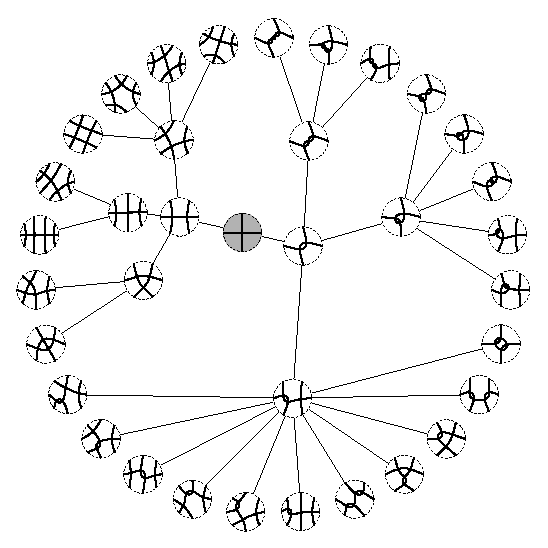
\includegraphics{c/genealogical-tree.eps}
			\caption{Дерево проекций\label{figure:genealogical-tree}}
		\end{figure}

		\begin{definition}
			Пусть $I$ --- проекция тангла, состоящая из единственного пререкрестка. Определим на множестве простых связных
			прекций $k$-танглов отображение $prev(T)$ следующим образом:
			\begin{itemize}
				\item
				$prev(I) = \varnothing$

				\item
				Для всех остальных $prev(T)$ будет являться результатом удаления из $T$ пограничного перекрестка $v$, не
				являющегося точкой сочленения, такого что root-code($T$, $v$) лексикографически минимален среди всех подобных
				перекрестков.
			\end{itemize}
		\end{definition}

		Согласно результатам параграфа~\ref{subsection:cutting}, отображение $prev(T)$ определено на всем множестве простых связных
		проекций $k$-танглов. Оно однозначно благодаря тому, что все удовлетворяющие определению способы выбора перекрестка отличаются
		друг от друга автоморфизмом (см. параграф~\ref{subsection:root-code}), следовательно все результаты удаления таких пограничных
		перекрестков гомеоморфны друг другу, а гомеоморфные проекции мы друг от друга не отличаем. И, наконец, оно обладает
		полуинвариантом --- числом перекрестков. Благодаря всем перечисленным свойствам, $prev(T)$ задает на множестве всех связных
		простых проекций структуру бесконечного дерева с корнем в $I$ (см.~\figureref{figure:genealogical-tree}).

		Таким образом, для перечисления всех проекций не более чем с $n$ перекрестками достаточно обойти это дерево DFS-ом на глубину
		не более, чем $n$ (см.~Алгоритм~\ref{algorithm:projections-enumeration}). Единственный тонкий момент, который мы должны
		учитывать --- это не спускаться по одному и тому же ребру несколько раз.

		\begin{algorithm}[ht]
			\caption{DFS(T)\label{algorithm:projections-enumeration}}
			\algsetup{linenosize=\small, linenodelimiter=.}
			\begin{algorithmic}[1]
				\PRINT $T$
				\IF{$crossings[T] = n$}
					\RETURN
				\ENDIF

				\STATE $list \leftarrow \varnothing$
				\FOR{(для) всех возможных результатов $R$ приклеивания перекрестка $v$ к $T$}
					\IF{$R$ --- простая}
						\IF{$prev(R) = T$}
							\STATE $r \leftarrow $ root-code($R$, $v$)
							\IF{ {\bf not} $contains(list, r)$}
								\STATE DFS($R$)
								\STATE $add(list, r)$
							\ENDIF
						\ENDIF
					\ENDIF
				\ENDFOR
			\end{algorithmic}
		\end{algorithm}

	\subsection{Результаты}

		Количества проекций $k$-танглов не более чем с 12 перекрестками, полученные в результате выполнения алгоритма, приведены
		в Таблице~\ref{table:tangle-projections}.

		\begin{landscape}
		\begin{table}[ht]
			\caption{Количество проекций $k$-танглов с $n$ перекрестками.\label{table:tangle-projections}}
			\centering
			\begin{tabular}{|c||r|r|r|r|r|r|r|r|r|r|r|r|}
			\hline
			$k$\textbackslash $n$
			    & 1 & 2 & 3 &  4 &   5 &   6 &      7 &       8 &        9 &          10 &           11 &            12 \\
			\hline\hline
			2   & 1 & 1 & 2 &  6 &  19 &  71 &    293 &  1\,348 &   6\,568 &     33\,701 &     178\,706 &      973\,085 \\
			3   & . & 1 & 2 &  8 &  29 & 138 &    638 &  3\,237 &  16\,805 &     90\,239 &     494\,151 &   2\,756\,453 \\
			4   & . & . & 2 &  8 &  41 & 210 & 1\,125 &  6\,138 &  34\,112 &    192\,278 &  1\,096\,560 &   6\,317\,363 \\
			5   & . & . & . &  5 &  31 & 231 & 1\,458 &  9\,183 &  56\,084 &    340\,885 &  2\,060\,224 &  12\,446\,400 \\
			6   & . & . & . &  . &  16 & 161 & 1\,406 & 10\,572 &  74\,331 &    499\,902 &  3\,276\,104 &  21\,112\,641 \\
			7   & . & . & . &  . &   . &  60 &    840 &  8\,818 &  75\,747 &    591\,091 &  4\,327\,816 &  30\,451\,898 \\
			8   & . & . & . &  . &   . &   . &    261 &  4\,702 &  56\,199 &    541\,570 &  4\,628\,641 &  36\,633\,417 \\
			9   & . & . & . &  . &   . &   . &      . &  1\,243 &  26\,753 &    361\,106 &  3\,846\,580 &  35\,758\,786 \\
			10  & . & . & . &  . &   . &   . &      . &       . &   6\,257 &    155\,593 &  2\,332\,512 &  27\,199\,662 \\
			11  & . & . & . &  . &   . &   . &      . &       . &        . &     32\,721 &     916\,595 &  15\,123\,600 \\
			12  & . & . & . &  . &   . &   . &      . &       . &        . &           . &     175\,760 &   5\,464\,661 \\
			13  & . & . & . &  . &   . &   . &      . &       . &        . &           . &            . &      963\,900 \\
			\hline
			все & 1 & 2 & 6 & 27 & 136 & 871 & 6\,021 & 45\,241 & 352\,856 & 2\,839\,086 & 23\,333\,649 & 195\,201\,866 \\
			\hline
			\end{tabular}
		\end{table}
		\end{landscape}

	\newpage
\section{Перечисление альтернированных $k$-танглов}
	\label{section:alternating}

	Для начала заметим, что в любой связной проекции существует только два способа расставить перекрестки альтернированным образом, которые
	мы различать не будем, так как они либо отвечают эквивалентным $k$-танглам, либо отличающимся только зеркальным отражением, которые мы
	тоже отождествляем. Таким образом, все альтернированные танглы мы будем рассматривать как подмножество проекций, содержащее по одному
	представителю из каждого класса эквивалентности по flype-преобразованиям.

	В данной главе мы обсудим генерацию связных простых альтернированных $k$-танглов на основе изложенного в предыдущей алгоритма генерации
	проекций. Однако теперь нам понадобится более сложный способ представления диаграмм, поэтому мы начнем с теоремы, следствиями которой
	будут важные свойства нового представления, описанного в параграфе~\ref{subsection:subtangle-decomposition}.

	\subsection{Теорема о пересекающихся танглах}

		Под словом ``тангл'' ниже будет подразумеваться простую связную диаграмму альтернированного $2$-тангла.

		\begin{theorem}
			\label{theorem:tangle-decomp-th}
			Пусть у нас есть два связных тангла $A$ и $B$, содержащиеся в какой-то простой альтернированной диаграмме
			тангла или зацепления $D$. При этом $A\setminus B\neq\varnothing$, $B\setminus A\neq\varnothing$
			и $A\cap B\neq\varnothing$. Тогда $A\setminus B$, $B\setminus A$, $A\cap B$ и $A\cup B$ --- также связные
			танглы, а $A\cup B$ представим в виде (см. \figureref{figure:tangle-decomp}):

			\begin{figure}[H]
				\centering
				\includegraphics{tangle-decomp-theorem.eps}
				\caption{К Теореме \ref{theorem:tangle-decomp-th}\label{figure:tangle-decomp}}
			\end{figure}
		\end{theorem}
		\begin{proof}
			Обозначим за $a$ количество ребер, ведущих из $A\setminus B$ в остальную часть $D$. Аналогично за $b$ и $c$
			обозначим количество ребер, ведущих в остальную часть $D$ из $B\setminus A$ и из $A\cup B$ соответственно.
			Буквами $d$, $e$ и $f$ обозначим количество ребер между $A\setminus B$ и $A\cup B$, между $B\setminus A$ и
			$A\cup B$ и между $A\setminus B$ и $B\setminus A$ соответственно (см. \figureref{figure:tangle-decomp-proof}).
			Так как $A$ и $B$ --- танглы, то выполняются соотношения:
			\begin{equation}
				\label{equation:a_relation}
				a + c + e + f = 4
			\end{equation}
			\begin{equation}
				\label{equation:b_relation}
				b + c + d + f = 4
			\end{equation}
			Из того, что диаграмма $D$ --- простая, а также из того, что у любого $k$-тангла четное количество ног, следует:
			\begin{equation}
				\label{equation:ab_relation}
				d + e + c \ge 4
			\end{equation}
			\begin{equation}
				\label{equation:all_relation}
				a + b + c \ge 4
			\end{equation}
			\begin{equation}
				\label{equation:amb_relation}
				a + d + f \ge 4
			\end{equation}
			\begin{equation}
				\label{equation:bma_relation}
				b + e + f \ge 4
			\end{equation}
			\begin{figure}[H]
				\centering
				\includegraphics{tangle-decomp-proof.eps}
				\caption{К доказательству Теоремы \ref{theorem:tangle-decomp-th}\label{figure:tangle-decomp-proof}}
			\end{figure}

			Складывая попарно (\ref{equation:a_relation}) и (\ref{equation:b_relation}),
			(\ref{equation:ab_relation}) и (\ref{equation:all_relation}),
			(\ref{equation:amb_relation}) и (\ref{equation:bma_relation}), получаем соответственно:
			\[a + b + d + e + 2c + 2f = 8\]
			\[a + b + d + e + 2c \ge 8\]
			\[a + b + d + e + 2f \ge 8\]
			Отсюда следует, что $c = f = 0$, а все нестрогие неравенства на самом деле являются равенствами. В результате
			получаем систему линейных уравнений на $a$, $b$, $d$ и $e$, единственным решением которой является
			$a = b = d = e = 2$. Завершим доказательство, заметив, что для связности $A\setminus B$, $B\setminus A$ и
			$A\cap B$ достаточно простоты $D$.
		\end{proof}


	\subsection{Разложение на $2$-танглы}
		\label{subsection:subtangle-decomposition}

		Каждая генерируемая диаграмма будет теперь представляться шаблоном --- специального вида проекцией $k$-тангла с таким же
		количеством концов и с меньшим количеством перекрестков, у которого в каждом перекрестке хранится дополнительная информация
		о том, какой из $2$-танглов нужно подставить вместо этого перекрестка, чтобы получить представляемую диаграмму. Похожая
		идея уже ранее использовалась в работе~\cite{SundbergThistlethwaite1998}.
		
		Так же, как и в старом алгоритме, мы будем получать диаграммы, последовательно склеивая их из перекрестков, но теперь разных
		типов перекрестков будет много --- в каждом может быть любой $2$-тангл $T$ любым из $\frac{|D_4|}{|G(T)|}$ способов. Здесь
		$G(T) \subset D_4$ --- група симметрий $2$-тангла $T$.

		Пусть у нас есть $k$-тангл $T$; мы хотим найти единственное разложение $T$ на максимальные $2$-танглы, то есть
		каждому перекрестку $v$ из $T$ сопоставить $2$-тангл $S(v) \subset T$ такой, что:
		\begin{list}{}{}
			\item $v \in S(v)$
			\item $\forall R \subset T$, где $R$ --- $2$-тангл, $v \in R \Rightarrow R \subset S(v)$
			\item $\forall u, u \in S(v) \Leftrightarrow S(u) = S(v)$
		\end{list}
		Заметим, что единственность такого разложения является следствием свойств, выполнения которых мы от него потребовали, а
		существование --- следствием Теоремы \ref{theorem:tangle-decomp-th}, если у исходного тангла имеется как минимум шесть
		концов. В случае же $2$-танглов содержательного (то есть не совпадающего со всем танглом) разложения на $2$-танглы
		может и не существовать. Подобные случаи мы рассмотрим далее.

		\begin{figure}[ht]
			\centering
			\def\pic#1{\raise-14mm\hbox{\includegraphics{tangle-decomp-example-#1.eps}}}
			$$\pic{1} \qquad \Rightarrow \qquad \pic{2}$$
			\caption{Разложение на $2$-танглы}
		\end{figure}

		Заметим, что ни какой flypе не меняет структуру шаблона. Также заметим, что при удалении из шаблона любого пограничного
		перекрестка, не являющегося точкой сочленения или его единственным перекрестком, в результате получается так же корректный
		шаблон какого-либо разложения. Единственное, что осталось сделать для того, чтобы получить весь набор $k$-танглов, имея
		изначально все $2$-танглы с информацией об их группах симметрии, это проверять по ходу склеивания, что у нас по-прежнему
		корректный шаблон, отсекая ``плохие'' ветки и обобщить наш инвариант на такие разложения. Первая задача легко решается
		нахождением минимального разреза, второй посвящен следующий параграф.

	\subsection{Инвариант разложений}

		Введем в каждом перекрестке шаблона $v$ функцию $tangle(v)$ --- неотрицательный номер содержащегося там $2$-тангла. При этом
		потребуем, чтобы у тангла из одного перекрестка был минимально возможный номер. Также введем функцию $orientation(v, e, f)$
		--- ориентацию содержащегося в $v$ $2$-тангла относительно входящего в $v$ ребра $e$ и направления обхода, заданного помеченной
		гранью $f$.

		\begin{algorithm}[ht]
			\caption{root-code-decomp$(P, (v, e, f))$\label{algorithm:root-code-decomp}}
			\algsetup{linenosize=\small, linenodelimiter=.}
			\begin{algorithmic}[1]
				\STATE $A \leftarrow \{\}$
				\STATE $free \leftarrow 2$

				\STATE $Q \leftarrow \{v\}$
				\STATE $number[v] \leftarrow 1$
				\STATE $incoming[v] \leftarrow e$

				\WHILE{$Q \neq \varnothing$}
					\STATE $u \leftarrow head[Q]$
					\STATE $dequeue(Q)$

					\STATE $push(A, tangle(u))$

					\FOR{(для) всех ребер $(u, w) \in P$ в порядке, заданном $f$, начиная с $incoming[u]$}
						\IF{$w$ --- конец диаграммы}
							\STATE $code \leftarrow 0$
						\ELSE
							\IF{$number[w]$ не определен}
								\STATE $number[w] \leftarrow free$
								\STATE $free \leftarrow free + 1$
								\STATE $enqueue(Q, w)$
							\ENDIF
							\STATE $code \leftarrow number[w]$
						\ENDIF

						\STATE $push(A, code)$
					\ENDFOR

					\STATE $push(A, orientation(u, incoming[u], f))$
				\ENDWHILE

				\RETURN $A$
			\end{algorithmic}
		\end{algorithm}

		Аналогично предыдущему определим root-code-decomp($P$, $v$). Заметим теперь, что инвариант, вычисленный в вершине, содержащей
		$2$-тангл из одного перекрестка, всегда будет лексикографиески меньше, чем вычисленный в вершине, содержащей что-то другое.

	\subsection{$2$-танглы}

		Теперь пришло время разобраться с предварительной генерацией $2$-танглов. Проблема с ними состоит в том, что не для каждого
		из них существует нетривиальное разложение. Сформулируем Теорему~\ref{theorem:tangle-sum-th}:

		\begin{theorem}
			\label{theorem:tangle-sum-th}
			Если для какого-то $2$-тангла $T$ не существует корректного разложения на $2$-танглы, то $T$ представим в виде прямой
			суммы двух или более $2$-танглов (см. Рис.~\ref{figure:tangle-sum}).

			\begin{figure}[H]
				\centering
				\includegraphics{tangle-sum.eps}
				\caption{Прямая сумма $T_1, T_2,\cdots, T_s$\label{figure:tangle-sum}}
			\end{figure}
		\end{theorem}
		\begin{proof}
			Если для $T$ не существует разложения на $2$-танглы, то в $T$ есть перекресток $v$ и собственные $2$-подтанглы $A$ и $B$
			такие, что $v \in A$, $v \in B$, $A\setminus B\neq\varnothing$, $B\setminus A\neq\varnothing$ и не существует такого
			собственного подтангла $T$, чтобы он содержал $A$ и $B$. Но по Теореме~\ref{theorem:tangle-decomp-th} $A \cup B$ ---
			$2$-тангл, следовательно $T = A \cup B$.
		\end{proof}
		
		Теорема~\ref{theorem:tangle-sum-th} позволяет однозначно разбить все $2$-танглы на две группы: допускающие разложение в прямую
		сумму и не допускающие. Для второй группы всегда существует корректное разложение на $2$-танглы, поэтому ее можно обрабатывать
		также, как и танглы с большим числом кончов. Разберемся теперь с первой группой.

		В нашем алгоритме танглы первой группы мы будем собирать из их слагаемых. При этом, для поддержания единственности разложения, ни
		одно из слагаемых не должно допускать дальнейшего разложения в прямую сумму в том же направлении. По ходу сборки за этим условием
		следить легко: для каждого $2$-тангла надо запомнить, раскладывается ли он в прямую сумму в этом направлении.

		\begin{figure}[ht]
			\centering
			\includegraphics{one-side-crossings.eps}
			\caption{Перекрестки с одной стороны.\label{figure:one-side-crossings}}
		\end{figure}

		С помощью flype-преобразований можно всегда добиться, чтобы все одиночные перекрестки находились в прямой сумме по одну сторону
		от остальных слагаемых (см.~\figureref{figure:one-side-crossings}) --- варианта их расположения всего два. В силу специфики
		устройства нашего инварианта, мы всегда добавляем к $2$-танглу, содержащему одиночный перекресток на границе только одиночные
		перекрестки, и ничего другого. Поэтому выбирать сторону, с которой будут расположены перекрестки надо только один раз при
		добавлении первого из них. Сделать это можно, сравнив значение инварианта в этих двух конфигурациях. Полностью правила
		сборки прямых сумм приведены в Таблице~\ref{table:sums-rules}.

		\begin{table}[ht]
			\caption{Правила сборки прямых сумм\label{table:sums-rules}}
			\centering
			\begin{tabular}{cm{22mm}l}
				\hline
				1 & \includegraphics{alternating-build-4-case-1.eps} & --- принять \\
				2 & \includegraphics{alternating-build-4-case-2.eps} & --- принять \\
				3 & \includegraphics{alternating-build-4-case-3.eps} & --- сравнить по root-code-decomp \\
				4 & \includegraphics{alternating-build-4-case-4.eps} & --- нарушается положение перекрестков \\
				5 & \includegraphics{alternating-build-4-case-5.eps} & --- нарушается положение перекрестков \\
				6 & \includegraphics{alternating-build-4-case-6.eps} & --- не бывает \\
				7 & \includegraphics{alternating-build-4-case-7.eps} & --- принять \\
				8 & \includegraphics{alternating-build-4-case-8.eps} & --- не бывает \\
				\hline
			\end{tabular}
		\end{table}

		Так как $2$-танглы, вообще говоря, могут обладать симметриями, связанными с поворотами, отражениями или flype-эквивалентностью,
		то согласно \figureref{figure:D4-subgroups} нужно вычислять их группы симметрии, являющиеся одной из 10 подгрупп $D_4$, анализируя
		результаты вычисления инвариантов с разными пометками.

		\begin{figure}
			\centering
			\includegraphics{d4-subgroups.eps}
			\caption{Подгруппы $D_4$.\label{figure:D4-subgroups}}
		\end{figure}

	\subsection{Результаты}

		В Таблице~\ref{table:old-results-table} приведены количества $2$-танглов без учета симметрии (то есть каждый $2$-тангл $T$ нужно
		учесть с весом $\frac{|D_4|}{|G(T)|}$). Результаты согласуются с~\cite{SundbergThistlethwaite1998}.

		\begin{table}[ht]
			\caption{Количество альтернированных $2$-танглов без учета поворотов и отражений.\label{table:old-results-table}}
			\centering
			\begin{tabular}{|r|r|r|r|r|r|r|r|r|r|r|r|}
			\hline
			1 & 2 & 3 &  4 &  5 &  6 &   7 &    8 &    9 &    10 &     11 &     12 \\
			\hline
			1 & 2 & 4 & 10 & 29 & 98 & 372 & 1538 & 6755 & 30996 & 146982 & 715120 \\
			\hline
			\end{tabular}
		\end{table}

		Изображения всех связных простых альтернированных $k$-танглов приведены на \figureref{figure:tangles14} и \figureref{figure:tangles5}.
		В Таблице~\ref{table:alternating-tangles-table} приведены их количества до 12 перекрестков.

		\begin{figure}[ht]
			\centering
			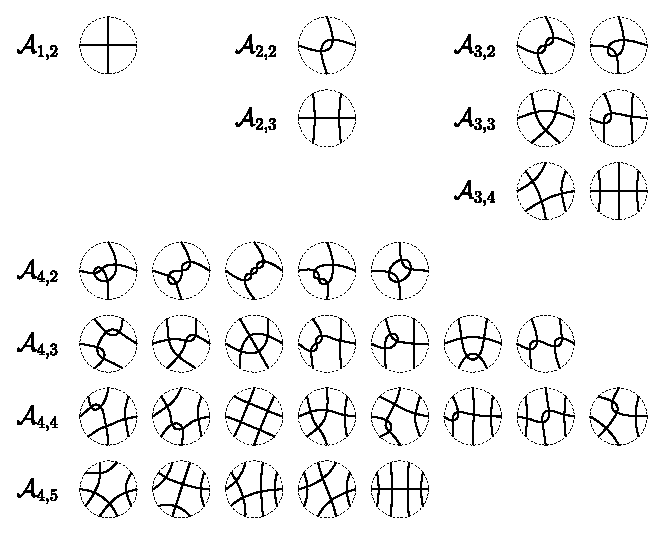
\includegraphics{c/alternating-tangles-1-4.eps}
			\caption{Альтернированные танглы до 4-х перекрестков\label{figure:tangles14}}
		\end{figure}

		\begin{figure}[ht]
			\centering
			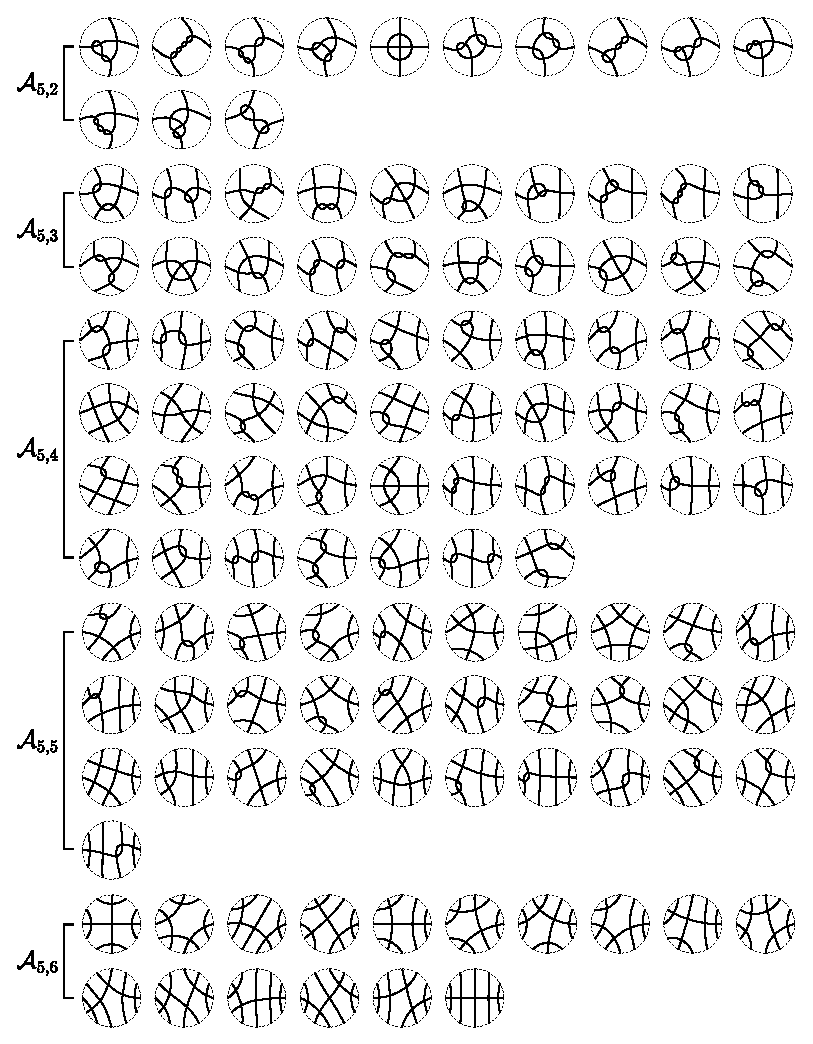
\includegraphics{c/alternating-tangles-5.eps}
			\caption{Альтернированные танглы c 5-ю перекрестками\label{figure:tangles5}}
		\end{figure}

		\begin{landscape}
		\begin{table}[ht]
			\caption{Количество альтернированных $k$-танглов с $n$ перекрестками.\label{table:alternating-tangles-table}}
			\centering
			\begin{tabular}{|c||r|r|r|r|r|r|r|r|r|r|r|r|}
			\hline
			$k$\textbackslash $n$
			    & 1 & 2 & 3 &  4 &   5 &   6 &      7 &       8 &        9 &          10 &           11 &            12 \\
			\hline\hline
			2   & 1 & 1 & 2 &  5 &  13 &  36 &    111 &     373 &   1\,362 &      5\,378 &      22\,807 &      102\,617 \\
			3   & . & 1 & 2 &  7 &  20 &  77 &    276 &  1\,135 &   4\,823 &     21\,734 &     101\,307 &      488\,093 \\
			4   & . & . & 2 &  8 &  37 & 157 &    687 &  3\,052 &  13\,981 &     65\,797 &     317\,506 &   1\,565\,163 \\
			5   & . & . & . &  5 &  31 & 209 & 1\,128 &  5\,986 &  30\,556 &    155\,964 &     795\,918 &   4\,092\,027 \\
			6   & . & . & . &  . &  16 & 161 & 1\,294 &  8\,528 &  51\,475 &    294\,366 &  1\,637\,855 &   8\,979\,493 \\
			7   & . & . & . &  . &   . &  60 &    840 &  8\,206 &  62\,895 &    428\,254 &  2\,702\,902 &  16\,313\,106 \\
			8   & . & . & . &  . &   . &   . &    261 &  4\,702 &  52\,815 &    460\,189 &  3\,475\,551 &  23\,979\,733 \\
			9   & . & . & . &  . &   . &   . &      . &  1\,243 &  26\,753 &    341\,878 &  3\,327\,424 &  27\,625\,056 \\
			10  & . & . & . &  . &   . &   . &      . &       . &   6\,257 &    155\,593 &  2\,221\,544 &  23\,869\,621 \\
			11  & . & . & . &  . &   . &   . &      . &       . &        . &     32\,721 &     916\,595 &  14\,473\,275 \\
			12  & . & . & . &  . &   . &   . &      . &       . &        . &           . &     175\,760 &   5\,464\,661 \\
			13  & . & . & . &  . &   . &   . &      . &       . &        . &           . &            . &      963\,900 \\
			\hline
			все & 1 & 2 & 6 & 25 & 117 & 700 & 4\,597 & 33\,225 & 250\,917 & 1\,961\,874 & 15\,695\,169 & 127\,916\,745 \\
			\hline
			\end{tabular}
		\end{table}
		\end{landscape}

	\newpage
\section{Алгоритмы рисования диаграмм $k$-танглов}
	\label{section:drawing}

	Общая идея подобных алгоритмов рисования выглядит следующим образом: мы кодируем картинку конечным
	набором чисел, а затем сопоставляем каждой такой конфигурации числовое значение энергии с помощью
	некоторого выбираемого из эстетических соображений отображения. Затем с помощью какого-либо метода
	оптимизации мы находим изображение, соответствующее минимальной энергии --- это и будет результатом.

	Однако, чтобы получить картинки хорошего качества, надо использовать достаточно сложную функцию
	энергии, нахождение глобального минимума которой, вообще говоря, весьма нетривиальная задача. Еще одной
	проблемой является требование изотопности картинки изображаемой конфигурации --- со сложной
	функцией гарантировать его выполнение в глобальном минимуме практически невозможно. Поэтому мы будем
	строить изображение в две стадии --- сначала, используя максимально простую энергетическую функцию,
	получим начальное приближение, а потом, уже со сложной функцией, улучшим его методом градиентного
	спуска.

	\begin{figure}[ht]
		\centering
		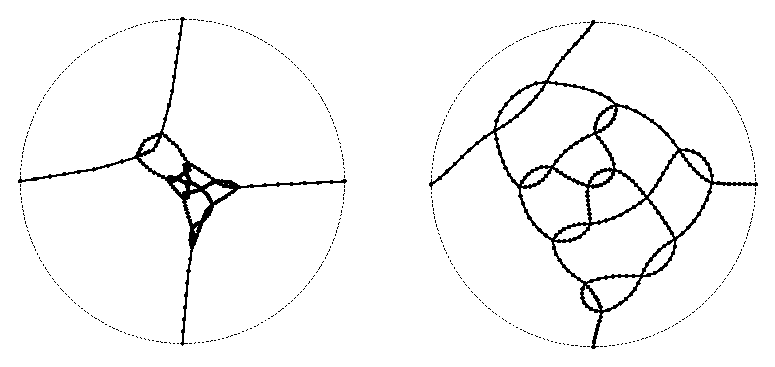
\includegraphics{c/drawing-energy.eps}
		\caption{Начальное приближение и градиентный спуск\label{figure:draw-optimization}}
	\end{figure}

	\subsection{Начальное приближение}

	На начальном этапе мы будем использовать простейшую возможную энергетическую функцию ---
	квадратичную форму
	$$
		E(x) = x \cdot Ax + b \cdot x
	$$
	Ее достоинствами являются простая физическая интерпретация как упругих взаимодействий и то, что минимум
	(если, конечно, он существует и единственен) легко найти из уравнения
	$$
		(A + A^T)x_{min} + b = 0
	$$

	Однако такой простейший подход, как выбрать в качестве переменных координаты перекрестков, а ребра представить
	упругими ``пружинками'' не приводит к желаемому результату (см.~\figureref{figure:degenerate-elastic}).
	\begin{figure}[ht]
		\centering
		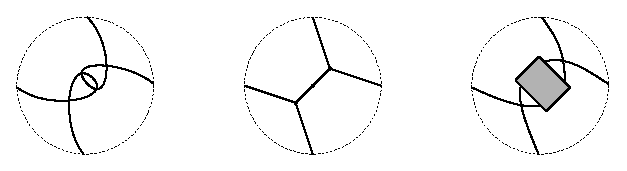
\includegraphics{c/drawing-initial-degeneration.eps}
		\caption{Диаграммы, вырождающиеся при утягивании\label{figure:degenerate-elastic}}
	\end{figure}

	Решить эту проблему можно при помощи добавления к графу дополнительных ребер-растяжек. Поместим в середину
	каждого исходного ребра тангла и каждой дуги границы-окружности дополнительный узел. Дополнительные узлы
	соединим между собой растяжками как показано на \figureref{figure:extra-elastic}. Можно представлять себе эти
	дополнительные ребра как стороны многоугольников, вписанных в грани исходного графа
	(\figureref{figure:extra-elastic}a), или же иначе --- как стяжки, попарно соединяющие соседние ребра, исходящие
	из каждой вершины тангла (\figureref{figure:extra-elastic}b).

	\begin{figure}[ht]
		\centering
		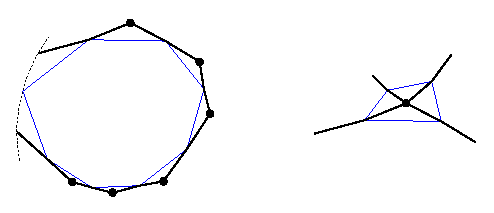
\includegraphics{c/drawing-face-crossing.eps}
		\caption{Дополнительные растяжки\label{figure:extra-elastic}}
	\end{figure}

	\begin{figure}[ht]
		\centering
		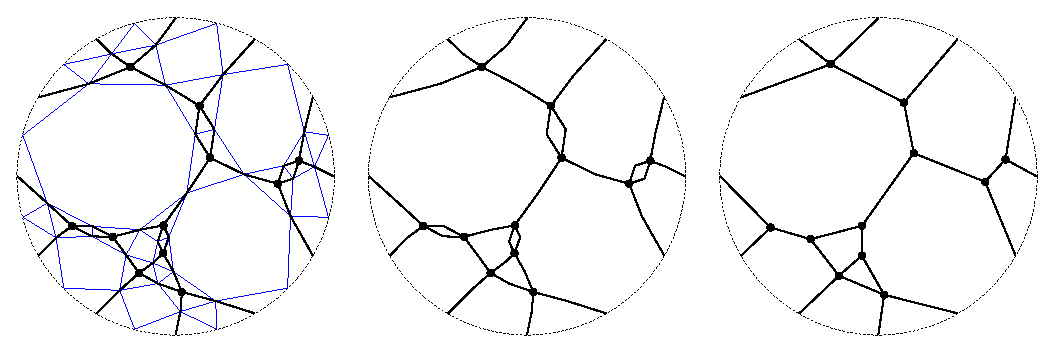
\includegraphics[scale=0.7]{c/drawing-initial-configuration-example.eps}
		\caption{Начальная конфигурация с растяжками и без\label{figure:startconfig}}
	\end{figure}

	При этом в каждой из 2-угольных граней мы получим две совпадающих растяжки. Оставим из них одну. Если у исходного
	тангла было $n$ перекрестков и $k$ концов, то полученный в результате граф содержит $n$ 4-валентных вершин
	(перекрестки исходного тангла), $k$ вершин валентности 2 (фиксированные дополнительные вершины на окружности)
	и $2n + k/2$ 5-6-валентных вершин (сколько ребер в графе тангла, 5-валентные вершины лежат на ребрах 2-угольных
	граней). Построим теперь для этого графа конфигурацию, соответствующую минимуму суммы квадратов длин ребер
	(см.~\figureref{figure:startconfig}).

	\subsection{Градиентный спуск}

	Второй стадией построения изображения, как и было сказано выше, является улучшение начальной конфигурации, полученной на
	предыдущем шаге. Для этого мы помещаем на каждом ребре начальной конфигурации еще по 1-2 промежуточных узла и запускаем
	метод градиентного спуска с новой более сложной энергетической функцией. В процессе мы должны следить за тем, чтобы за
	одну итерацию не происходило слишком больших прыжков, могущих изменить топологию текущей конфигурации, то есть ограничивать
	большие прыжки сверху.

	Основные требования к функционалу энергии для градиентного спуска:
	\begin{enumerate}
		\item
		бесконечный потенциальный барьер, препятствующий прохождению узлов через звенья;

		\item
		обращение в бесконечность при наложении ребер и стягивании в точку граней графа;

		\item
		непрерывность касательных в перекрестках;

		\item
		сходимость при увеличении числа точек на ребро;

		\item
		эстетические критерии --- хорошая различимость всех перекрестков и примерно равномерное распределение их в круге,
		длины ребер примерно равны, углы в перекрестках близки к прямым, плавное изменение кривизны
	\end{enumerate}

	Предлагаемая энергетическая функция будет линейной комбинацией четырех компонент: электростатического отталкивания элементов
	диаграммы друг от друга, электростатического отталкивания от граничной окружности, силы упругости ребер и ``изгибной''
	энергии, стремящейся спрямлять картинку в вершинах степени 2 и добиваться перпендикулярности входящих ребер в вершинах
	степени 4.

	Энергия электростатического отталкивания типа ``узел-узел'' не удовлетворяет самому важному требованию --- не обеспечивает
	потенциального барьера изменению топологии. Кроме того, рельеф потенциальной функции изобилует ямами. Энергия отталкивания
	типа ``звено-звено'' обеспечивает барьер, однако выражается довольно громоздкими формулами. Есть также проблема с вычислением
	сил взаимодействия сцепленных (инцидентных одной вершине) ребер. Наиболее подходящей кажется смешанная энергия ``звено-узел''.
	Будем считать, что заряд равномерно распределен по длине ребер тангла с единичной плотностью, но силы отталкивания сосредоточены
	в узлах, заряды которых пропорциональны полусумме длин соседних ребер. Такая схема соответствует вычислению повторного интеграла
	энергии при помощи смешанной квадратурной формулы --- одно интегрирование выполняется методом трапеций, а другое --- методом
	центральных прямоугольников.
	\begin{figure}[ht]
		\centering
		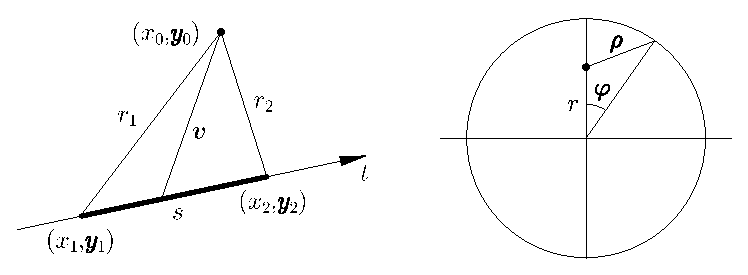
\includegraphics{c/drawing-energy-definition.eps}
		\caption{К определению электростатического потенциала взаимодействия\label{figure:electrostatic}}
	\end{figure}
	Электростатический потенциал, создаваемый заряженным отрезком (см.~\figureref{figure:electrostatic}):
	\begin{eqnarray*}
		\phi(x_0, y_0)
		= \int_0^s\frac{dt}{|\vec{v}|}
		= s\int_0^1\frac{d\tau}{\bigl([\xi_1(1-\tau)+\xi_2\tau]^2+[\eta_1(1-\tau)+\eta_2\tau]^2\bigr)^{1/2}} = {}\\
		= \ln\biggl(\frac{r_1+r_2+s}{r_1+r_2-s}\biggr)
	\end{eqnarray*}
	Здесь $\xi_{1,2}=x_0-x_{1,2}$, $\eta_{1,2}=y_0-y_{1,2}$; остальные обозначения приведены на~\figureref{figure:electrostatic}.

	Электростатический потенциал заряженной окружности единичного радиуса в ее плоскости (см.~~\figureref{figure:electrostatic}):
	$$
		\phi(r)=2\int_0^{\pi}\frac{d\phi}{\rho}=\frac{4}{1+r}\mathsf{K}\Bigl(\frac{4r}{(1+r)^2}\Bigr),
	$$
	где $\mathsf{K}()$ --- полный эллиптический интеграл 1-го рода.

	Изгибную энергию введем следующим образом. Для ломаной, заданной вершинами $p_k$, построим в каждой вершине векторы, равные
	сумме исходящих из данной вершины векторов звеньев (см.~\figureref{figure:bend-energy}). Определим изгибную энергию ломаной
	как сумму квадратов длин полученных векторов:
	$$
		E=\sum_k (x_{k-1}-2x_k+x_{k+1})^2+(y_{k-1}-2y_k+y_{k+1})^2
	$$
	Здесь $x_k$, $y_k$ --- координаты вершины $p_k$ ломаной.
	\begin{figure}[ht]
		\centering
		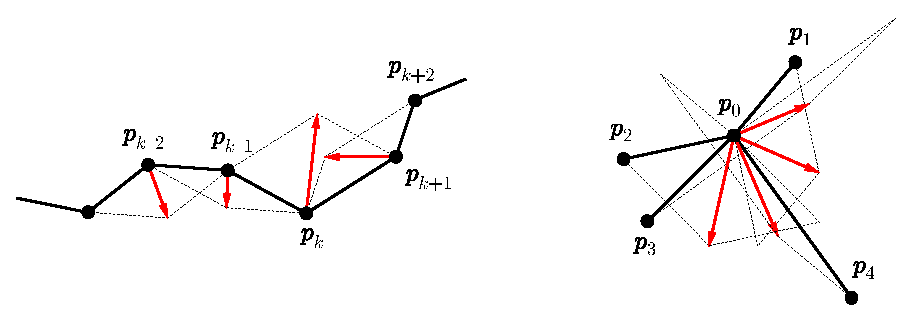
\includegraphics{c/drawing-bend-energy.eps}
		\caption{К определению изгибной энергии\label{figure:bend-energy}}
	\end{figure}
	Такая изгибная энергия равна нулю только для равнозвенной прямолинейной ломаной. Компоненты градиента изгибной энергии представляют
	собой разности 4-го порядка последовательности координат вершин:
	\begin{eqnarray*}
		\frac{\partial E}{\partial x_k} = x_{k-2} - 4x_{k-1} + 6x_k - 4x_{k+1} + x_{k+2} \\ [10pt]
		\frac{\partial E}{\partial y_k} = y_{k-2} - 4y_{k-1} + 6y_k - 4y_{k+1} + y_{k+2}
	\end{eqnarray*}

	Аналогичную функцию можно использовать для того чтобы выполнить еще одно требование к ``хорошо нарисованной'' проекции --- дуги в
	перекрестках должны пересекаться под приблизительно прямым углом. Обозначим узлы, соседние с данным перекрестком, в порядке против
	часовой стрелки, $p_1$, $p_2$, $p_3$ и $p_4$ (см.~\figureref{figure:bend-energy}) и введем соответствующие векторы, исходящие из
	перекрестка: $(x_1 - x_0, y_1 - y_0)$ и т.д. Мерой перпендикулярности двух последовательных векторов может служить вектор --- сумма
	одного из них с перпендикулярной копией второго. Энергию перекрестка определим как сумму квадратов длин таких векторов:
	\begin{eqnarray*}
		E = (x_2-x_0+y_1-y_0)^2 + (y_2-y_0-x_1+x_0)^2 + (x_3-x_0+y_2-y_0)^2 + \\
		+ (y_3-y_0-x_2+x_0)^2 + (x_4-x_0+y_3-y_0)^2 + (y_4-y_0-x_3+x_0)^2 + \\
		+ (x_1-x_0+y_4-y_0)^2 + (y_1-y_0-x_4+x_0)^2
	\end{eqnarray*}
	Это выражение обращается в ноль лишь когда все четыре вектора равны по величине, и все углы прямые.

	\newpage
\section{Заключение}
	Все известные алгоритмы перечисления объектов теории узлов работают похожим образом: сначала каким-то образом генерируются
	все ``интересные'' диаграммы исследуемых объектов, затем с помощью определенных инвариантов и хеш-таблиц из полученного
	множества диаграмм удаляются повторы, соответствующие одному и тому же объекту. Например, в процессе перечисления альтернированных
	зацеплений в \cite{Rankin2002_1, Rankin2002_2, Rankin2002_3} для генерации диаграмм использовались локальные преобразования,
	как на \figureref{figure:surgeries}, а удаление дубликатов производилось с помощью введенного авторами полного инварианта
	``Master Array''.
	\begin{figure}[ht]
		\centering
		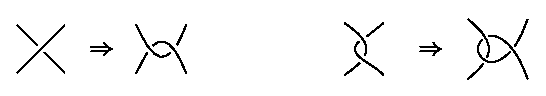
\includegraphics{c/surgeries.eps}
		\caption{Локальные преобразования\label{figure:surgeries}}
	\end{figure}

	Очевидным недостатком такой схемы являются необходимость поддерживать хеш-таблицу очень больших размеров и выполнять поиск
	по ней. Также часто возникает проблема с тем, что доля заведомо бесполезной работы с увеличением размера объектов возрастает
	экспоненциально, так как экспоненциально растет доля повторяющихся диаграмм. Предложенный в данной работе тип алгоритмов
	свободен от подобного рода проблем. Перебор проекций в Главе~\ref{section:projections} вообще не требует хранения уже
	полученных им объектов, а алогоритм генерации альтернированных $k$-танглов из Главы~\ref{section:alternating} не требует
	поиска и хранит только малую часть сгенерированного. Доля лишней работы растет не более чем линейно с ростом максимального
	числа концов.

	Еще одним достоинством предложенной схемы является широкая возможность ее обобщения. В качестве примера, легко понять как
	приспособить ее для генерации полимино, или диаграмм альтернированных зацеплений, или, возможно, самих альтернированных
	зацеплений.

	Вероятным следующим шагом могло бы явится обобщение алгоритма на неальтернированные $k$-танглы, впрочем в этом случае такое
	свойство, как отсутствие поисковых запросов по уже сгенерированным объектам, скорее всего не удастся сохранить.

	Реализации на языке C++ приведенных алгоритмов можно найти по адресу \uline{http://code.google.com/p/tanglenum/}.

	\newpage
\renewcommand{\bibname}{Список литературы}
\begin{thebibliography}{99}
	\addcontentsline{toc}{section}{\bibname}

	\bibitem{Conway1970}
	Conway J. An enumeration of knots and links, and some of their algebraic
	properties. Computational Problems in Abstract Algebra (John Leech, ed.), Pergamon Press, Oxford
	and New York, 1969, 329-358.

	\bibitem{Cromwell2004}
	Cromwell P. Knots and links. Cambridge: Cambridje university press. 2004. 350~p.

	\bibitem{KanenobuSaitoSatoh2003}
	Kanenobu T., Saito H., and Satoh S. Tangles with up to seven crossings.
	Interdisciplinary Information Sciences, Vol. 9, No. 1, pp. 127-140 (2003).

	\bibitem{KauffmanLambropoulou2004}
	Kauffman L., Lambropoulou S. On the classification of rational tangles.
	Advances in Applied Mathematics Volume 33, Issue 2, August 2004, Pages 199-237.
	e-print:~\texttt{arXiv:math/0311499v2}

	\bibitem{Justin1999_1}
	Zinn-Justin P. Matrix Integrals and the Counting of Tangles and Links.
	e-print:~\texttt{arXiv:math-ph/9904019v2}

	\bibitem{Justin1999_2}
	Zinn-Justin P. Some Matrix Integrals related to Knots and Links
	e-print:~\texttt{arXiv:math-ph/9910010v1}

	\bibitem{JustinZuber2000}
	Zinn-Justin P., Zuber J. On the Counting of Colored Tangles.
	e-print:~\texttt{arXiv:math-ph/0002020v2}

	\bibitem{Justin2001}
	Zinn-Justin P. The General O(n) Quartic Matrix Model and its application to Counting Tangles and Links.
	e-print:~\texttt{arXiv:math-ph/0106005v1}

	\bibitem{JacobsenJustin2002}
	Jacobsen J.L., Zinn-Justin P. The combinatorics of alternating tangles:
	from theory to computerized enumeration. e-print:~\texttt{arXiv:math-ph/0111011v1}

	\bibitem{JustinZuber2003}
	Zinn-Justin P., Zuber J. Matrix integrals and the generation and counting
	of virtual tangles and links. J.Knot Theor.Ramifications 13 (2004) 325-356.
	e-print:~\texttt{arXiv:math-ph/0303049}

	\bibitem{Kauffman1999}
	Kauffman L. Virtual knot theory. European Journal of Combinatorics. 1999.
	20. P.663--690.  e-print:~\texttt{arXiv:math/9811028v3}

	\bibitem{Kuperberg2003}
	Kuperberg G. What is a virtual link? Algebr. Geom. Topol. 3 (2003) 587--591.
	e-print:~\texttt{arXiv:math/0208039v2}

	\bibitem{Tait1900}
	Tait, P.G. On Knots I, II, III. Scientific Papers, Vol. 1. London: Cambridge University Press, pp. 273--347, 1900.

	\bibitem{MenascoThistlethwaite1991}
	Menasco, W. and Thistlethwaite, M. The Tait Flyping Conjecture. Bull. Amer. Math. Soc. 25, 403--412, 1991. 

	\bibitem{MenascoThistlethwaite1993}
	Menasco, W. and Thistlethwaite, M. The Classification of Alternating Links. Ann. Math. 138, 113--171, 1993.

	\bibitem{SundbergThistlethwaite1998}
	Sundberg, C. and Thistlethwaite, M. The Rate of Growth of the Number of Prime Alternating Links and Tangles.
	Pacific Journal of Mathematics, Vol. 182, No. 2, pp. 329--358, 1998.

	\bibitem{Rankin2002_1}
	Rankin S., Schermann J., Smith O. Enumerating the prime alternating knots, Part	I,
	Journal of Knot Theory and Its Ramifications, Vol. 13, No. 1 (2004) 57-100
	e-print:~\texttt{arXiv:math/0211346}

	\bibitem{Rankin2002_2}
	Rankin S., Schermann J., Smith O. Enumerating the prime alternating knots, Part II,
	Journal of Knot Theory and Its Ramifications, Vol. 13, No. 1 (2004) 101-149
	e-print:~\texttt{arXiv:math/0211348}

	\bibitem{Rankin2002_3}
	Rankin S., Smith O. Enumerating the Prime Alternating Links
	Journal of Knot Theory and Its Ramifications, Vol. 13, No. 1 (2004) 151-173
	e-print:~\texttt{arXiv:math/0211451}

\end{thebibliography}

\end{document}
